% Options for packages loaded elsewhere
\PassOptionsToPackage{unicode}{hyperref}
\PassOptionsToPackage{hyphens}{url}
%
\documentclass[
]{book}
\title{Medidas de diversidade}
\author{Fabio Cop Ferreira \and \href{mailto:fabiocopf@gmail.com}{\nolinkurl{fabiocopf@gmail.com}}; \href{mailto:fcferreira@unifesp.br}{\nolinkurl{fcferreira@unifesp.br}} \and Instituto do Mar, Universidade Federal de São Paulo}
\date{Última atualização em 12/12/2021}

\usepackage{amsmath,amssymb}
\usepackage{lmodern}
\usepackage{iftex}
\ifPDFTeX
  \usepackage[T1]{fontenc}
  \usepackage[utf8]{inputenc}
  \usepackage{textcomp} % provide euro and other symbols
\else % if luatex or xetex
  \usepackage{unicode-math}
  \defaultfontfeatures{Scale=MatchLowercase}
  \defaultfontfeatures[\rmfamily]{Ligatures=TeX,Scale=1}
\fi
% Use upquote if available, for straight quotes in verbatim environments
\IfFileExists{upquote.sty}{\usepackage{upquote}}{}
\IfFileExists{microtype.sty}{% use microtype if available
  \usepackage[]{microtype}
  \UseMicrotypeSet[protrusion]{basicmath} % disable protrusion for tt fonts
}{}
\makeatletter
\@ifundefined{KOMAClassName}{% if non-KOMA class
  \IfFileExists{parskip.sty}{%
    \usepackage{parskip}
  }{% else
    \setlength{\parindent}{0pt}
    \setlength{\parskip}{6pt plus 2pt minus 1pt}}
}{% if KOMA class
  \KOMAoptions{parskip=half}}
\makeatother
\usepackage{xcolor}
\IfFileExists{xurl.sty}{\usepackage{xurl}}{} % add URL line breaks if available
\IfFileExists{bookmark.sty}{\usepackage{bookmark}}{\usepackage{hyperref}}
\hypersetup{
  pdftitle={Medidas de diversidade},
  pdfauthor={Fabio Cop Ferreira; fabiocopf@gmail.com; fcferreira@unifesp.br; Instituto do Mar, Universidade Federal de São Paulo},
  hidelinks,
  pdfcreator={LaTeX via pandoc}}
\urlstyle{same} % disable monospaced font for URLs
\usepackage{color}
\usepackage{fancyvrb}
\newcommand{\VerbBar}{|}
\newcommand{\VERB}{\Verb[commandchars=\\\{\}]}
\DefineVerbatimEnvironment{Highlighting}{Verbatim}{commandchars=\\\{\}}
% Add ',fontsize=\small' for more characters per line
\usepackage{framed}
\definecolor{shadecolor}{RGB}{248,248,248}
\newenvironment{Shaded}{\begin{snugshade}}{\end{snugshade}}
\newcommand{\AlertTok}[1]{\textcolor[rgb]{0.94,0.16,0.16}{#1}}
\newcommand{\AnnotationTok}[1]{\textcolor[rgb]{0.56,0.35,0.01}{\textbf{\textit{#1}}}}
\newcommand{\AttributeTok}[1]{\textcolor[rgb]{0.77,0.63,0.00}{#1}}
\newcommand{\BaseNTok}[1]{\textcolor[rgb]{0.00,0.00,0.81}{#1}}
\newcommand{\BuiltInTok}[1]{#1}
\newcommand{\CharTok}[1]{\textcolor[rgb]{0.31,0.60,0.02}{#1}}
\newcommand{\CommentTok}[1]{\textcolor[rgb]{0.56,0.35,0.01}{\textit{#1}}}
\newcommand{\CommentVarTok}[1]{\textcolor[rgb]{0.56,0.35,0.01}{\textbf{\textit{#1}}}}
\newcommand{\ConstantTok}[1]{\textcolor[rgb]{0.00,0.00,0.00}{#1}}
\newcommand{\ControlFlowTok}[1]{\textcolor[rgb]{0.13,0.29,0.53}{\textbf{#1}}}
\newcommand{\DataTypeTok}[1]{\textcolor[rgb]{0.13,0.29,0.53}{#1}}
\newcommand{\DecValTok}[1]{\textcolor[rgb]{0.00,0.00,0.81}{#1}}
\newcommand{\DocumentationTok}[1]{\textcolor[rgb]{0.56,0.35,0.01}{\textbf{\textit{#1}}}}
\newcommand{\ErrorTok}[1]{\textcolor[rgb]{0.64,0.00,0.00}{\textbf{#1}}}
\newcommand{\ExtensionTok}[1]{#1}
\newcommand{\FloatTok}[1]{\textcolor[rgb]{0.00,0.00,0.81}{#1}}
\newcommand{\FunctionTok}[1]{\textcolor[rgb]{0.00,0.00,0.00}{#1}}
\newcommand{\ImportTok}[1]{#1}
\newcommand{\InformationTok}[1]{\textcolor[rgb]{0.56,0.35,0.01}{\textbf{\textit{#1}}}}
\newcommand{\KeywordTok}[1]{\textcolor[rgb]{0.13,0.29,0.53}{\textbf{#1}}}
\newcommand{\NormalTok}[1]{#1}
\newcommand{\OperatorTok}[1]{\textcolor[rgb]{0.81,0.36,0.00}{\textbf{#1}}}
\newcommand{\OtherTok}[1]{\textcolor[rgb]{0.56,0.35,0.01}{#1}}
\newcommand{\PreprocessorTok}[1]{\textcolor[rgb]{0.56,0.35,0.01}{\textit{#1}}}
\newcommand{\RegionMarkerTok}[1]{#1}
\newcommand{\SpecialCharTok}[1]{\textcolor[rgb]{0.00,0.00,0.00}{#1}}
\newcommand{\SpecialStringTok}[1]{\textcolor[rgb]{0.31,0.60,0.02}{#1}}
\newcommand{\StringTok}[1]{\textcolor[rgb]{0.31,0.60,0.02}{#1}}
\newcommand{\VariableTok}[1]{\textcolor[rgb]{0.00,0.00,0.00}{#1}}
\newcommand{\VerbatimStringTok}[1]{\textcolor[rgb]{0.31,0.60,0.02}{#1}}
\newcommand{\WarningTok}[1]{\textcolor[rgb]{0.56,0.35,0.01}{\textbf{\textit{#1}}}}
\usepackage{longtable,booktabs,array}
\usepackage{calc} % for calculating minipage widths
% Correct order of tables after \paragraph or \subparagraph
\usepackage{etoolbox}
\makeatletter
\patchcmd\longtable{\par}{\if@noskipsec\mbox{}\fi\par}{}{}
\makeatother
% Allow footnotes in longtable head/foot
\IfFileExists{footnotehyper.sty}{\usepackage{footnotehyper}}{\usepackage{footnote}}
\makesavenoteenv{longtable}
\usepackage{graphicx}
\makeatletter
\def\maxwidth{\ifdim\Gin@nat@width>\linewidth\linewidth\else\Gin@nat@width\fi}
\def\maxheight{\ifdim\Gin@nat@height>\textheight\textheight\else\Gin@nat@height\fi}
\makeatother
% Scale images if necessary, so that they will not overflow the page
% margins by default, and it is still possible to overwrite the defaults
% using explicit options in \includegraphics[width, height, ...]{}
\setkeys{Gin}{width=\maxwidth,height=\maxheight,keepaspectratio}
% Set default figure placement to htbp
\makeatletter
\def\fps@figure{htbp}
\makeatother
\setlength{\emergencystretch}{3em} % prevent overfull lines
\providecommand{\tightlist}{%
  \setlength{\itemsep}{0pt}\setlength{\parskip}{0pt}}
\setcounter{secnumdepth}{5}
\usepackage{booktabs}
\usepackage{amsthm}
\makeatletter
\def\thm@space@setup{%
  \thm@preskip=8pt plus 2pt minus 4pt
  \thm@postskip=\thm@preskip
}
\makeatother
\usepackage{booktabs}
\usepackage{longtable}
\usepackage{array}
\usepackage{multirow}
\usepackage{wrapfig}
\usepackage{float}
\usepackage{colortbl}
\usepackage{pdflscape}
\usepackage{tabu}
\usepackage{threeparttable}
\usepackage{threeparttablex}
\usepackage[normalem]{ulem}
\usepackage{makecell}
\usepackage{xcolor}
\ifLuaTeX
  \usepackage{selnolig}  % disable illegal ligatures
\fi
\usepackage[]{natbib}
\bibliographystyle{apalike}

\begin{document}
\maketitle

{
\setcounter{tocdepth}{1}
\tableofcontents
}
\hypertarget{uxedndice}{%
\chapter*{Índice}\label{uxedndice}}
\addcontentsline{toc}{chapter}{Índice}

\hypertarget{part-medidas-de-diversidade}{%
\part{Medidas de diversidade}\label{part-medidas-de-diversidade}}

\hypertarget{introdiversidade}{%
\chapter{Medidas de diversidade: introdução}\label{introdiversidade}}

Geralmente entendemos por \emph{diverso}, um ambiente em que existem muitas espécies. Uma floresta tropical é um ambiente mais diverso que uma floresta temperada e um trecho de mata atlântica mais diverso que um ambientre desértico, pois os primeiros contém mais espécies. O número de espécies existentes em uma região, denominado de \textbf{riqueza de espécies (S)} é um componente fundamental da diversidade em comunidades ecológicas.

Considere as duas comunidades abaixo:

\begin{center}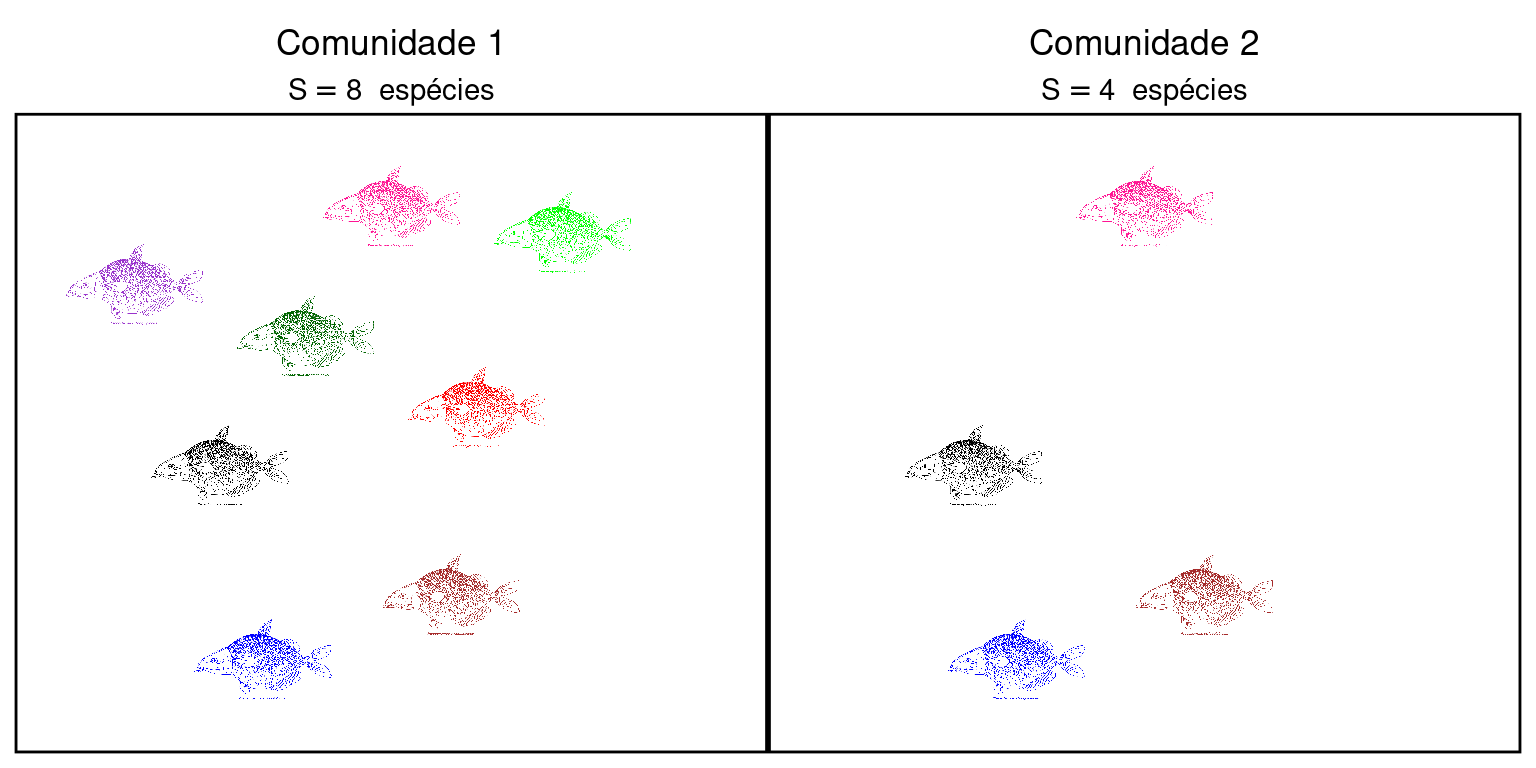
\includegraphics{medidas-diversidade_files/figure-latex/unnamed-chunk-4-1} \end{center}

Se medirmos a diversidade de uma comunidade por meio da riqueza de espécies, a comunidade \(1\) (\(S = 8\)) é duas vezes mais diversa que a comunidade \(2\) (\(S = 4\)). Entretanto, outro componente fundamental do que compreendemos por diversidade de espécies tem relação com o \textbf{grau de uniformidade} ou \textbf{equabilidade} das abundâncias relativas. Se duas comunidades têm a mesma riqueza, será mais diversa aquela em que as abundâncias relativas forem mais uniformes entre as espécies.

Suponha duas comunidades com \(5\) espécies e \(100\) indivíduos. Na comunidade A todas as espécies têm \(20\) indivíduos, enquanto na comunidade B, a espécie mais abundante tem \(96\) indivíduos e todas as restantes somente \(1\) indivíduo cada. A comunidade A será mais diversa pois tem uma distribuição de abundância relativa mais uniforme, enquanto a segunda comunidade é menos uniforme pois apresenta elevada \textbf{dominância}.

Ao combinarmos estes dois componentes podemos encontrar diferentes tipos de comunidades: i - comunidades com baixa riqueza de espécies e baixa dominância, ii - comunidades com baixa riqueza de espécies e alta dominância; iii - comunidades com alta riqueza de espécies e baixa dominância ou iii - comunidades com alta riqueza de espécies e alta dominância.

\begin{center}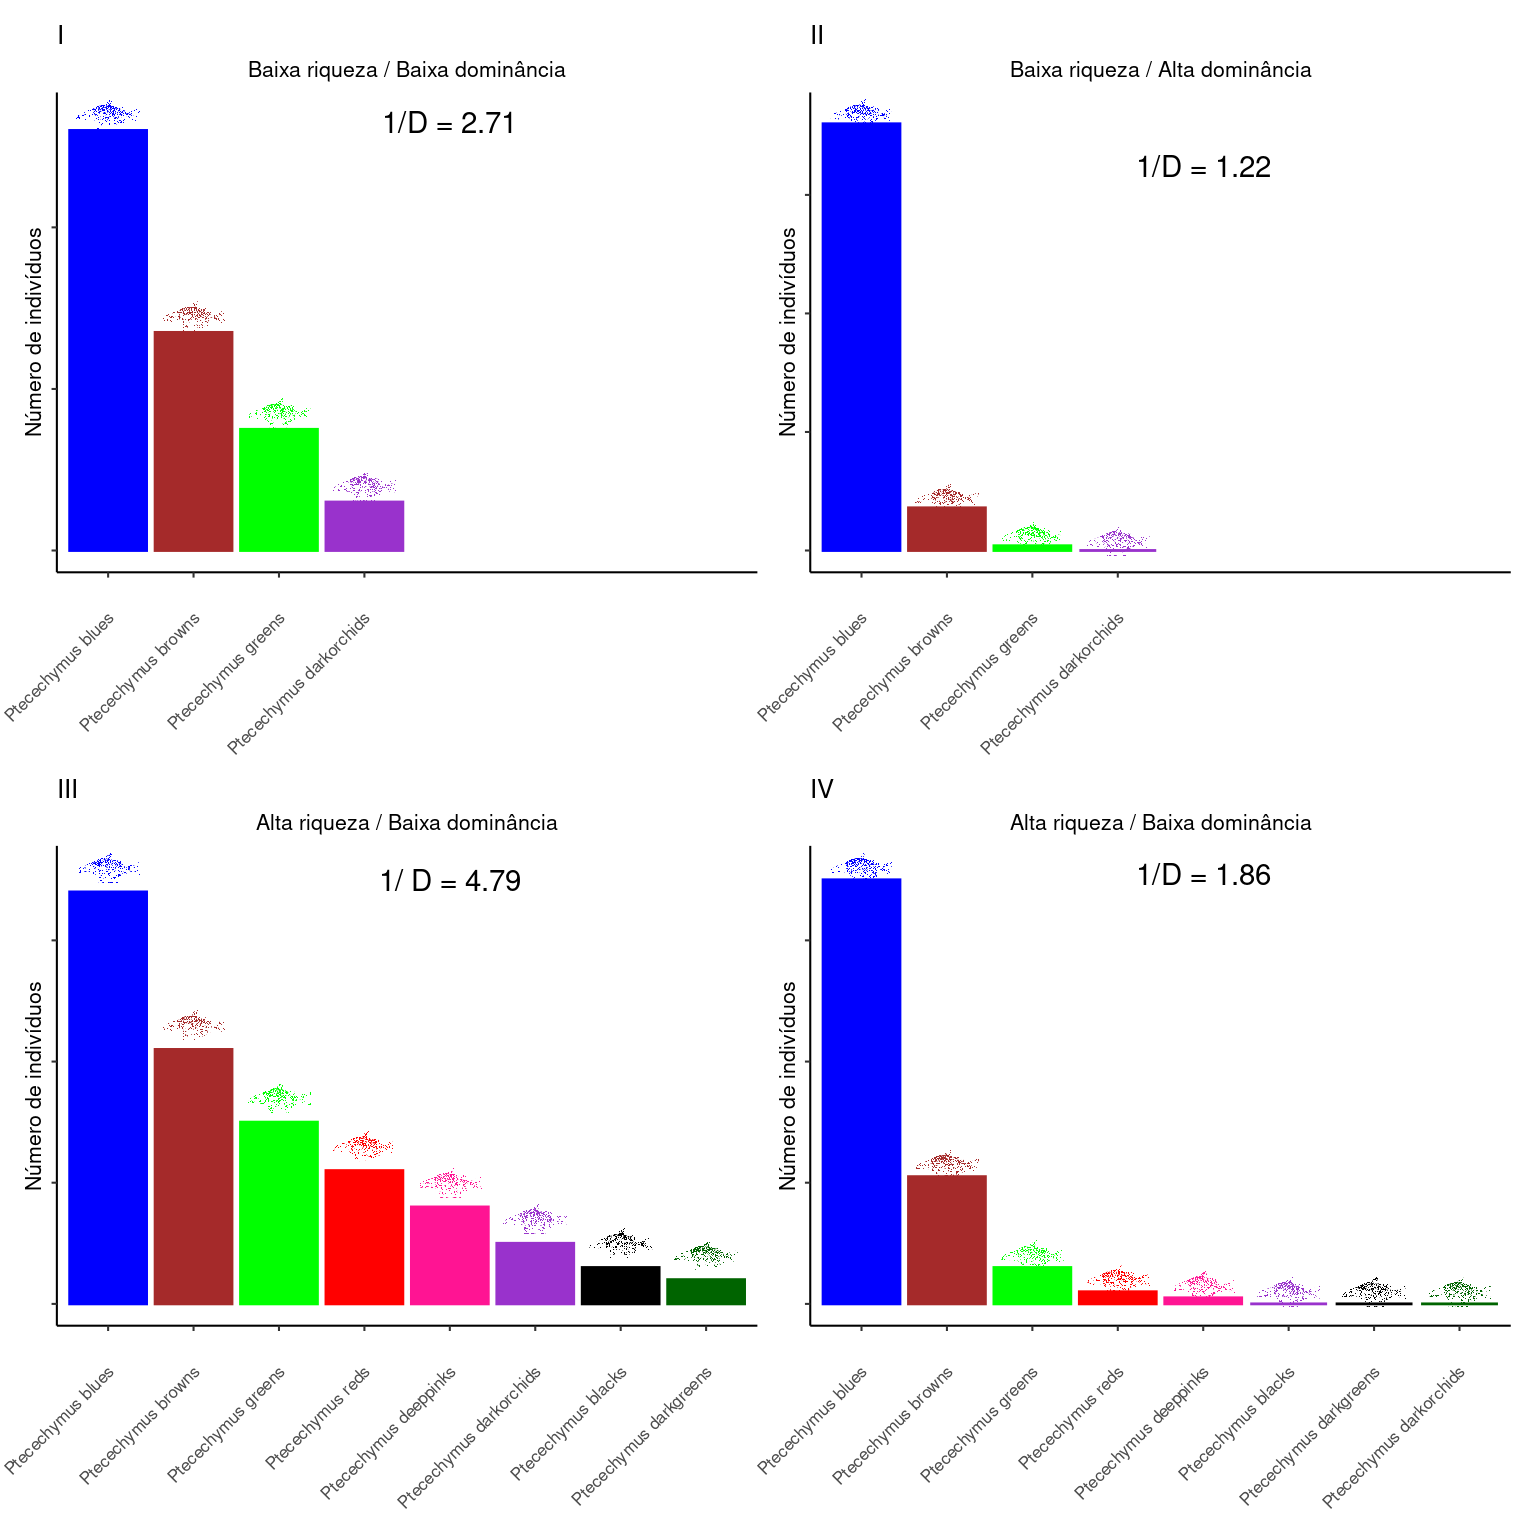
\includegraphics{medidas-diversidade_files/figure-latex/unnamed-chunk-7-1} \end{center}

\hypertarget{indices-de-diversidade}{%
\section{Indices de diversidade}\label{indices-de-diversidade}}

Os índices de diversidade capturam os dois componentes (riqueza de espécies e uniformidade) em uma única medida. Neste sentido, um elevado valor de diversidade pode ocorrer devido à elevada riqueza ou a elevada uniformidade (= baixa dominância).

Abaixo irei descrever um deles, com propriedades bem conhecidas: o \textbf{índice de Simpson}.

\textbf{Índice de diversidade de Simpson}

Simpson (1949 - Measurement of diversity) definiu uma medida de diversidade a partir da probabilidade de que dois indivíduos retirados aleatoriamente de uma comunidade fossem pertencentes à mesma espécie. Para uma comunidade com número finito de indivíduos esta probabilidade pode ser dada por:

\[D = \sum_{i = 1}^{S}\left(\frac{n_i(n_1 - 1)}{N(N-1)}\right)\]

Se existe uma alta dominância, é \textbf{altamente provavel} que dois indivíduos retirados ao acaso sejam da mesma espécie. Deste modo, \(D\) dimuniu quando a comunidade é muito diversa. Para resolver esta questão comumente representado o índice de diversidade de Simpson por \(1 - D\) ou \(1/D\). O índice de Simpson captura a variância na distribuição de abundância da espécie, sobretudo para valores de riqueza acima de \(10\) espécies (Maguran, 2004).

Para as comunidades representadas nas figuras acima temos:

\begin{itemize}
\item
  Comunidade I: \(1 - D = 0.63\)
\item
  Comunidade II: \(1 - D = 0.18\)
\item
  Comunidade III: \(1 - D = 0.79\)
\item
  Comunidade IV: \(1 - D = 0.46\)
\end{itemize}

A comunidade \(III\) é a mais diversa pois possui elevada riqueza e alta uniformidade, enquanto a comunidade \(II\) é a menos diversa pois possui menor riqueza e baixa uniformidade. Finalmente, as comunidades \(I\) e \(IV\) ficam no meio do caminho pois possuem baixa riqueza mas alta uniformidade ou vice-versa.

\textbf{Índice de Equabilidade de Simpson}

Uma vez que \(D\) combina riqueza com uniformidade, poderíamos buscar uma medida que evidenciasse somente a última (uma vez que a riqueza é simples de se obter). Se utilizarmos a diversidade de Simpson, teríamos a medida de \textbf{equabilidade de Simpson} como:

\[E_{1/D} = \frac{1/D}{S}\]

\(E_{1/D}\) varia entre \(0\) e \(1\) e não é sensível á riqueza de espécies.

Existe uma variedade de índices de diversidade e equabilidade. Para uma apresentação detalhada \citet{magurran2011medindo} e uma discussão da relação entre riqueza, diversidade e equabilidade veja \citet{melo2008ganhamos} (acesse aqui).

\hypertarget{diversidade-na-paisagem}{%
\section{Diversidade na paisagem}\label{diversidade-na-paisagem}}

Ao olharmos para uma paisagem perceberemos que invariavelmente, há algum grau de variabilidade na estrutura ambiental, sendo possivel muitas vezes reconhecer \textbf{manchas de habitats}. Considere riachos em uma bacia costeira típica do litoral de São Paulo. Podemos encontar trechos com estruturas de hábitats altamente variáveis em termos tipo de substrato (rochoso \emph{vs} arenoso), largura, velocidade de corrente, sombreamento, etc.

\begin{center}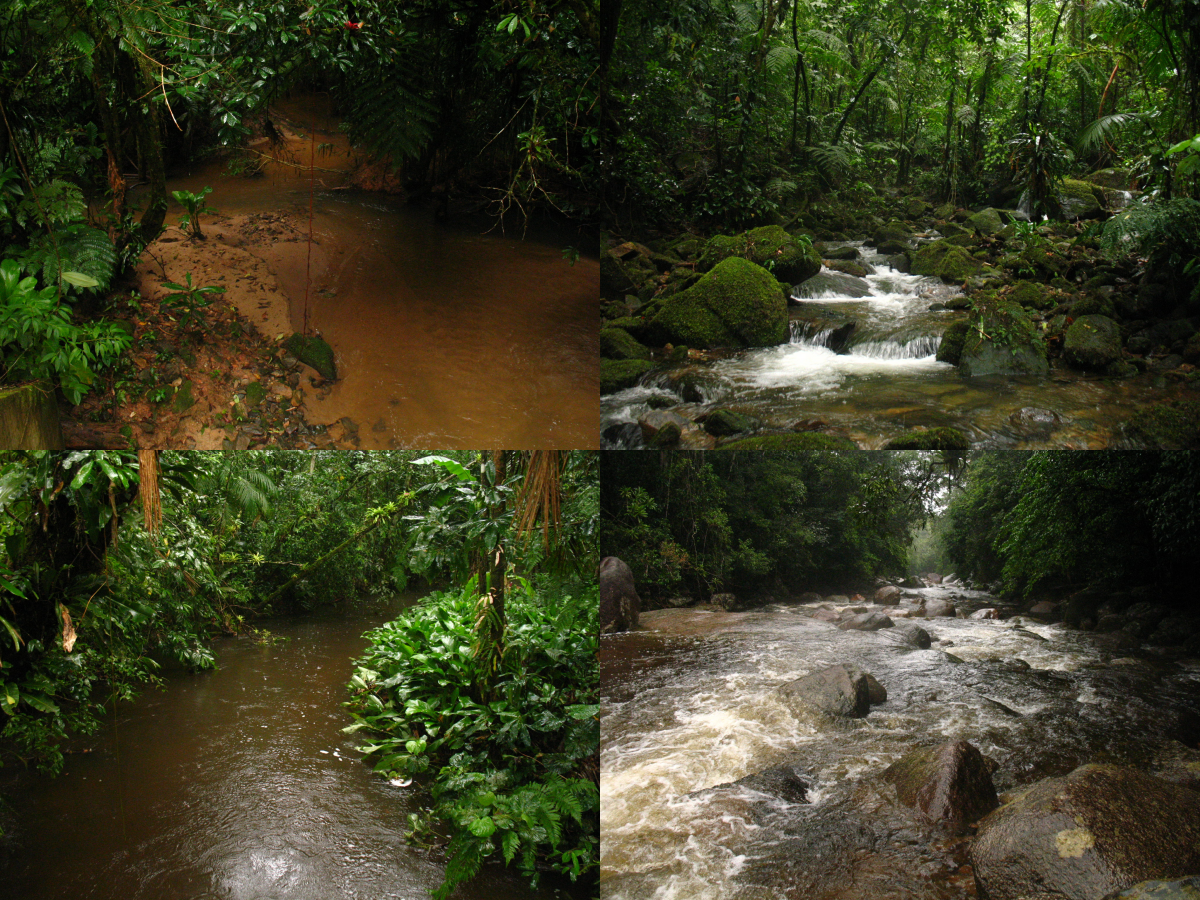
\includegraphics[width=16.67in]{medidas-diversidade_files/figure-latex/unnamed-chunk-8-1} \end{center}

É esperado que a composição de espécies presentes em cada um destes locais seja diferente, o que levará a variações nos padrões de riqueza e uniformidade das comunidades. O mesmo vale para qualquer ambiente em que seja possível verificar alguma variação espacial na estrutura dos habitats. Algumas destas variações ocorrem em forma de gradiente ambiental. Por exemplo, há um gradiente de umidade e de exposição às ondas que vai do trecho superior (supral-itoral) ao trecho inferior (infra-litoral) de faixas de areia em praias. É esperado que a fauna que habite estes ambientes varie ao longo deste gradiente.

Mesmo que não haja um gradiente ambiental forte, ainda é esperado que devido à dinâmicas individuais de nascimento, morte, imigração, emigração, as espécies se distribuam de forma heterogênea na paisagem. Portanto, se queremos caracterizar a diveridade em uma determinada região, devemos amostrar diferentes parcelas na paisagem, o que nos leva a buscar reconhecer padrões de diversidade em diferentes escalas.

Se tivermos na paisagem uma \(5\) comunidades diferentes, cada um com \(5\) espécies sem nenhuma sobreposição, a diversidade da paisagem será maior (\(S = 25\)) que as diversidades locais (\(S = 5\)).

Se por outro lado, todas as comunidades tiverem exatamente as mesmas espécies, ao combiná-las, ainda teremos \(S = 5\) espécies na paisagem.

Muitas vezes não é possivel amostrar um hábitat por completo (por exemplo, toda a faixa de areia), ou ainda pode não ser possível sequer reconhecer manchas de hábitas. Ainda assim, o protocolo de amostragem será composto por umnidades amostrais que se combinam para formar a amostra completa.

Imagine a amostragem de peixes na zona de arrebentação de praia da Baía de Santos. Cada amostra consiste do arrasto ao longo de \(200\) m. Ainda que não seja possível reconhecer limites físcos comunidades encontradas em cada unidade amostral, continua válida a ideia de que a diversidade na Baía de Santos será composta da combinação entre as comunidades provinientes de cada arrasto.

\begin{center}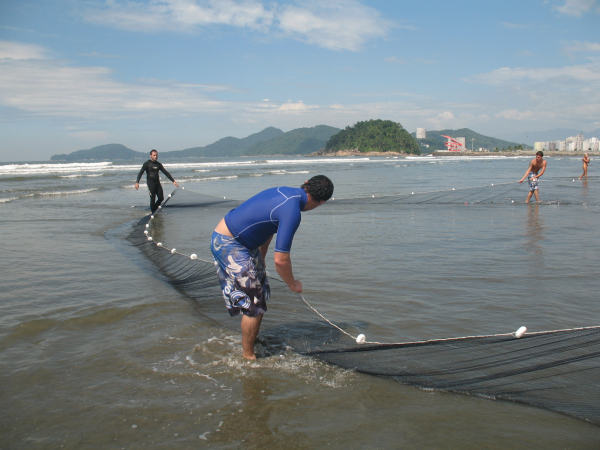
\includegraphics[width=8.33in]{medidas-diversidade_files/figure-latex/unnamed-chunk-9-1} \end{center}

Para organizar a diversidade em diferentes escalas, defini-se como diversidade \textbf{alfa (\(\alpha\))} a diversidade de uma única unidade amostral e como diversidade \textbf{gama (\(\gamma\))} a combinação detodas as diversidades locais na paisagem.

\begin{figure}

{\centering 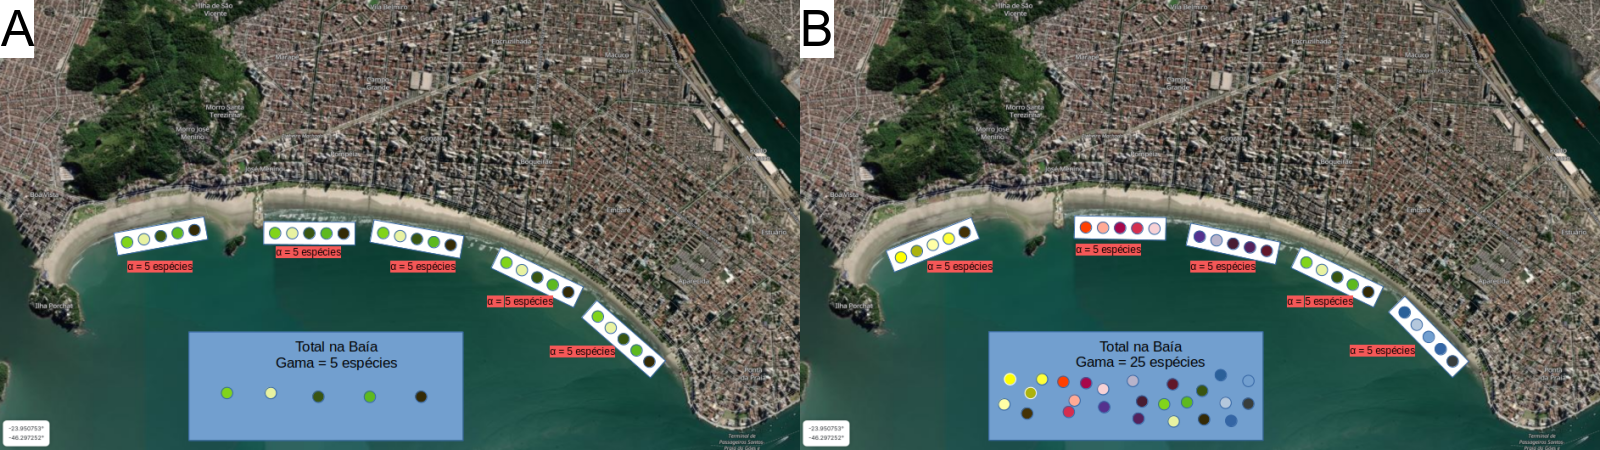
\includegraphics[width=22.22in]{medidas-diversidade_files/figure-latex/unnamed-chunk-10-1} 

}

\caption{A: Diversidade gama total (5 espécies) igual alfa locais (5 espécies). B: Diversidade gama total (25 espécies) maior alfa locais (5 espécies).}\label{fig:unnamed-chunk-10}
\end{figure}

Acima na figura da esquerda (Figura 1.1A) temos cinco amostras, cada uma contendo as mesmas \(5\) espécies. Ao combinarmos todas as amostras ainda teremos as mesmas espécies, de modo que as diversidades \(\alpha = \gamma = 5\) espécies.

Na figura da direita (Figura 1.1B) também temos cinco amostras, porém cada uma contém \(5\) espécies totalmente diferentes das demais amostras. Neste caso, a diversidade na paisagem será \(\gamma = 25\) espécies, enquanto as doversidades locais conterão \(\alpha = 5\) espécies.

Para diferenciar situações destes tipo definimos a \textbf{beta (\(\beta\))} que mede a diferença entre as diversidades \(\alpha\) e \(\gamma\). Nos exemplos acima temos portanto que a Figura 1.1A descreve uma situação com \textbf{baixa diversidade \(\beta\)}, enquanto a Figura 1.1B descreve uma situação com \textbf{alta diversidade \(\beta\)}

No capítulo seguinte iremos descrever como podemos medir e compreender a diversidade de espécies nas diferentes escalas.

\hypertarget{diversidader}{%
\chapter{\texorpdfstring{Medindo as diversidades \(\alpha\), \(\beta\) e \(\gamma\)}{Medindo as diversidades \textbackslash alpha, \textbackslash beta e \textbackslash gamma}}\label{diversidader}}

A tabela abaixo mostra a abundância de \(10\) peixes captradas na zona de arrebentação da Baís de Santos em 2015. Cada linha da tabela representa uma amostra, isto é, um arrasto feito ao longo de \(200\) m na zona de arrebentação das ondas seguindo a direção da linha da costa. No total foram \(12\) amostras. A primeira coluna identifica em que período do ano cada amostra foi obtida. As primeiras 6 foram tomadas no VERAO de \(2015\) e as outras 6 no INVERNO de \(2015\). As demais colunas mostram o número de indivíduos de cada espécie obtido nas amostras. Os nomes das espécies foram omitidos para facilitar a apresentação dos dados.

Vamos utilizar esta tabela como exemplo para calcularmos as diversidades \(\alpha\), \(\beta\) e \(\gamma\).

Os cálculos serão feitos no programa R. Antes de iniciar, é importante preparar seu ambiente de trabalho. Iremos utilizar o R-Studio como ambiente de programação, mas você pode utilizar outro de sua vontade. A seguir faremos toda a preparação necessárias, mas pode ser útil consultar os links abaixo:

\begin{itemize}
\item
  Introdução ao Ambiente R de Programação - Capítulos 1 e 2
\item
  Estatística nas Ciências Ambientais - Capítulos 2 e 11
\end{itemize}

\hypertarget{preparando-o-ambiente-de-trabalho}{%
\section{Preparando o ambiente de trabalho}\label{preparando-o-ambiente-de-trabalho}}

\begin{enumerate}
\def\labelenumi{\arabic{enumi}.}
\tightlist
\item
  Após abrir o R-Studio e criar um arquivo, direcionane R para a pasta de trabalho em quie você irá trabalhar. Por exemplo:
\end{enumerate}

\begin{Shaded}
\begin{Highlighting}[]
\FunctionTok{setwd}\NormalTok{(}\StringTok{\textquotesingle{}C:/Users/usuario/Documents/Bio\_II\_2021\textquotesingle{}}\NormalTok{ )}
\end{Highlighting}
\end{Shaded}

\begin{enumerate}
\def\labelenumi{\arabic{enumi}.}
\setcounter{enumi}{1}
\item
  Faça o download da base de dados (\textbf{arqivo .xlsx}) que iremos utilizar e salve na pasta que você selecionou acima. O arquivo está disponível para download no link Baia\_santos.xlsx
\item
  Caso ainda não tenha feito, instales os segintes pacotes com o comando abaixo:
\end{enumerate}

\begin{Shaded}
\begin{Highlighting}[]
\FunctionTok{install.packages}\NormalTok{(}\FunctionTok{c}\NormalTok{(}\StringTok{\textquotesingle{}tidyverse\textquotesingle{}}\NormalTok{, }\StringTok{\textquotesingle{}vegan\textquotesingle{}}\NormalTok{, }\StringTok{\textquotesingle{}patchwork\textquotesingle{}}\NormalTok{, }\StringTok{\textquotesingle{}readxl\textquotesingle{}}\NormalTok{, }\StringTok{\textquotesingle{}iNEXT\textquotesingle{}}\NormalTok{))}
\end{Highlighting}
\end{Shaded}

\begin{enumerate}
\def\labelenumi{\arabic{enumi}.}
\setcounter{enumi}{3}
\tightlist
\item
  E habilite os pacotes
\end{enumerate}

\begin{Shaded}
\begin{Highlighting}[]
\FunctionTok{library}\NormalTok{(tidyverse)}
\FunctionTok{library}\NormalTok{(vegan)}
\FunctionTok{library}\NormalTok{(patchwork)}
\FunctionTok{library}\NormalTok{(readxl)}
\FunctionTok{library}\NormalTok{(iNEXT)}
\end{Highlighting}
\end{Shaded}

\begin{quote}
Os pacotes precisam ser instalados somente uma vez. No entanto, sempre que você fechar e abrir o R-Studio, precisará habilitá-los novamente.
\end{quote}

\begin{enumerate}
\def\labelenumi{\arabic{enumi}.}
\setcounter{enumi}{4}
\tightlist
\item
  Importe a base de dados para o R-Studio
\end{enumerate}

\begin{Shaded}
\begin{Highlighting}[]
\NormalTok{pe }\OtherTok{=} \FunctionTok{read\_excel}\NormalTok{(}\StringTok{\textquotesingle{}Baia\_santos.xlsx\textquotesingle{}}\NormalTok{)}
\end{Highlighting}
\end{Shaded}

Após importar visualize a tabela:

\begin{Shaded}
\begin{Highlighting}[]
\FunctionTok{View}\NormalTok{(pe)}
\end{Highlighting}
\end{Shaded}

E verifique se as colunas foram lidas corretamente. Digite o comando abaixo:

\begin{Shaded}
\begin{Highlighting}[]
\FunctionTok{glimpse}\NormalTok{(pe)}
\end{Highlighting}
\end{Shaded}

\begin{verbatim}
## Rows: 12
## Columns: 11
## $ Epoca <chr> "INVERNO", "INVERNO", "INVERNO", "INVERNO", "INVERNO", "INVERNO"~
## $ sp_1  <dbl> 5, 6, 7, 0, 2, 0, 1, 0, 8, 2, 1, 1
## $ sp_2  <dbl> 6, 0, 0, 0, 0, 0, 0, 0, 0, 0, 0, 0
## $ sp_3  <dbl> 72, 1, 0, 0, 143, 95, 0, 0, 0, 0, 0, 0
## $ sp_4  <dbl> 65, 18, 48, 13, 48, 28, 8, 1, 1, 0, 3, 0
## $ sp_5  <dbl> 8, 9, 2, 4, 1, 0, 0, 3, 4, 6, 0, 0
## $ sp_6  <dbl> 6, 12, 0, 1, 0, 0, 27, 2, 6, 2, 2, 7
## $ sp_7  <dbl> 1, 0, 0, 0, 0, 1, 0, 2, 0, 0, 0, 0
## $ sp_8  <dbl> 0, 1, 4, 0, 1, 0, 0, 0, 0, 0, 0, 0
## $ sp_9  <dbl> 0, 0, 0, 0, 0, 0, 1, 0, 4, 0, 1, 0
## $ sp_10 <dbl> 0, 0, 0, 0, 0, 0, 0, 0, 0, 0, 0, 1
\end{verbatim}

Você deve ver uma saída parecida com esta. Verifique se \texttt{Epoca} aparace com o símbolo \texttt{\textless{}chr\textgreater{}}, indicando que é uma variável categórica e se todas as demais aparecem com o símbolo \texttt{\textless{}dbl\textgreater{}}, indicando que são variáveis quantitativas. Caso alguma variável (exceto \texttt{Epoca}) apareça como \texttt{\textless{}chr\textgreater{}} voce deve verificar em sua base de dados se existe algum caracter não numérico nas colunas das espécies.

\hypertarget{diversidade-alpha}{%
\section{\texorpdfstring{Diversidade \(\alpha\)}{Diversidade \textbackslash alpha}}\label{diversidade-alpha}}

A diversidade \(\alpha\) se refere às diversidades registradas localente,isto é, em cada uma das amostras. Após obtermos estas medidas, nos interessa entender qual a diversidade média. Como dizemos no capítulo anterior, a diversidade pode ser caracterizada por diferentes índices. Os dois componentes principais do que entendermos por diversidade são: \textbf{riqueza de espécies} e \textbf{equabilidade} (ou uniformidade). O primeiro refere-se simplesmente ao número de espécies em uma amostra. Se contarmos o número de espécies presentes na primeira linha da tabela por exemplo, encontraremos \(7\) espécies (sp\_1, sp\_2, sp\_3, sp\_4, sp\_5, sp\_6, sp\_7). Já na última amostra encontramos somente \(3\) espécies (sp\_1, sp\_6, sp\_10).

O segundo componente da diversidade se refere ao padrão de distribuição das abundâncias relativas. Se todas as espécies forem \emph{igualmente} abundantes, a uniformidade é máxima. Por outro lado, se uma ou poucas espécies são muito abundantes e todas as demais raras (compostas por poucos indivíduos), a uniformidade é baixa (= dominância alta). Na linha \(3\) por exemplo, uma das espécies é composta por \(48\) individuos, enquanto a segunda espécie mais abundante apareceu com somente \(7\).

Os índices de diversidade combinam a riqueza de espécies e equabilidade, para nos fonecer uma medida-resumo para as comunidades locais.

Como temos amostras tomadas em dois períodos nos interessa justamente comparar estes períodos em função das medidas de diversidade nas diferentes escalas.

\begin{tabular}{l|r|r|r|r|r|r|r|r|r|r}
\hline
Epoca & sp\_1 & sp\_2 & sp\_3 & sp\_4 & sp\_5 & sp\_6 & sp\_7 & sp\_8 & sp\_9 & sp\_10\\
\hline
INVERNO & 5 & 6 & 72 & 65 & 8 & 6 & 1 & 0 & 0 & 0\\
\hline
INVERNO & 6 & 0 & 1 & 18 & 9 & 12 & 0 & 1 & 0 & 0\\
\hline
INVERNO & 7 & 0 & 0 & 48 & 2 & 0 & 0 & 4 & 0 & 0\\
\hline
INVERNO & 0 & 0 & 0 & 13 & 4 & 1 & 0 & 0 & 0 & 0\\
\hline
INVERNO & 2 & 0 & 143 & 48 & 1 & 0 & 0 & 1 & 0 & 0\\
\hline
INVERNO & 0 & 0 & 95 & 28 & 0 & 0 & 1 & 0 & 0 & 0\\
\hline
VERAO & 1 & 0 & 0 & 8 & 0 & 27 & 0 & 0 & 1 & 0\\
\hline
VERAO & 0 & 0 & 0 & 1 & 3 & 2 & 2 & 0 & 0 & 0\\
\hline
VERAO & 8 & 0 & 0 & 1 & 4 & 6 & 0 & 0 & 4 & 0\\
\hline
VERAO & 2 & 0 & 0 & 0 & 6 & 2 & 0 & 0 & 0 & 0\\
\hline
VERAO & 1 & 0 & 0 & 3 & 0 & 2 & 0 & 0 & 1 & 0\\
\hline
VERAO & 1 & 0 & 0 & 0 & 0 & 7 & 0 & 0 & 0 & 1\\
\hline
\end{tabular}

Vamos adicionar ao final da tabela \texttt{pe} três colunas, uma com a riqueza de espécies (\(S\)), uma com o índice de diversidade de Simpson (\(D\)) e outra com a equabilidade de Simpson (\(E\)). Desta forma teremos os três componentes de diversidade.

\begin{Shaded}
\begin{Highlighting}[]
\NormalTok{pe }\OtherTok{=}\NormalTok{ pe }\SpecialCharTok{\%\textgreater{}\%}
  \FunctionTok{rowwise}\NormalTok{() }\SpecialCharTok{\%\textgreater{}\%} 
  \FunctionTok{mutate}\NormalTok{(}\AttributeTok{S =} \FunctionTok{specnumber}\NormalTok{(}\FunctionTok{c\_across}\NormalTok{(sp\_1}\SpecialCharTok{:}\NormalTok{sp\_10)),}
         \AttributeTok{D =} \FunctionTok{diversity}\NormalTok{(}\FunctionTok{c\_across}\NormalTok{(sp\_1}\SpecialCharTok{:}\NormalTok{sp\_10), }
                       \AttributeTok{index =} \StringTok{\textquotesingle{}invsimpson\textquotesingle{}}\NormalTok{)) }\SpecialCharTok{\%\textgreater{}\%} 
  \FunctionTok{mutate}\NormalTok{(}\AttributeTok{E =}\NormalTok{ D}\SpecialCharTok{/}\NormalTok{S)}
\end{Highlighting}
\end{Shaded}

Ao digitar a tabela novamente verá as três novas colunas criadas.

\begin{Shaded}
\begin{Highlighting}[]
\FunctionTok{View}\NormalTok{(pe)}
\end{Highlighting}
\end{Shaded}

\begin{table}
\centering\begingroup\fontsize{10}{12}\selectfont

\begin{tabular}{l|r|r|r|r|r|r|r|r|r|r|r|r|r}
\hline
Epoca & sp\_1 & sp\_2 & sp\_3 & sp\_4 & sp\_5 & sp\_6 & sp\_7 & sp\_8 & sp\_9 & sp\_10 & S & D & E\\
\hline
INVERNO & 5 & 6 & 72 & 65 & 8 & 6 & 1 & 0 & 0 & 0 & 7 & 2.775990 & 0.3965700\\
\hline
INVERNO & 6 & 0 & 1 & 18 & 9 & 12 & 0 & 1 & 0 & 0 & 6 & 3.763203 & 0.6272005\\
\hline
INVERNO & 7 & 0 & 0 & 48 & 2 & 0 & 0 & 4 & 0 & 0 & 4 & 1.568057 & 0.3920143\\
\hline
INVERNO & 0 & 0 & 0 & 13 & 4 & 1 & 0 & 0 & 0 & 0 & 3 & 1.741936 & 0.5806452\\
\hline
INVERNO & 2 & 0 & 143 & 48 & 1 & 0 & 0 & 1 & 0 & 0 & 5 & 1.670768 & 0.3341535\\
\hline
INVERNO & 0 & 0 & 95 & 28 & 0 & 0 & 1 & 0 & 0 & 0 & 3 & 1.567380 & 0.5224601\\
\hline
VERAO & 1 & 0 & 0 & 8 & 0 & 27 & 0 & 0 & 1 & 0 & 4 & 1.722013 & 0.4305031\\
\hline
VERAO & 0 & 0 & 0 & 1 & 3 & 2 & 2 & 0 & 0 & 0 & 4 & 3.555556 & 0.8888889\\
\hline
VERAO & 8 & 0 & 0 & 1 & 4 & 6 & 0 & 0 & 4 & 0 & 5 & 3.977444 & 0.7954887\\
\hline
VERAO & 2 & 0 & 0 & 0 & 6 & 2 & 0 & 0 & 0 & 0 & 3 & 2.272727 & 0.7575758\\
\hline
VERAO & 1 & 0 & 0 & 3 & 0 & 2 & 0 & 0 & 1 & 0 & 4 & 3.266667 & 0.8166667\\
\hline
VERAO & 1 & 0 & 0 & 0 & 0 & 7 & 0 & 0 & 0 & 1 & 3 & 1.588235 & 0.5294118\\
\hline
\end{tabular}
\endgroup{}
\end{table}

Veja que para cada amostra foi calculado um valor de \(S\), \(D\) e \(E\). A riqueza varia entre \(6\) e \(10\). Nenhuma amostra sozinha contém as \(10\) espécies totais encontradas na Baia.

\begin{quote}
Para manter a notação simples, estamos utilizando a simbologia \(D\) mas, extritamente falando, o argumento \texttt{index\ =\ \textquotesingle{}invsimpson\textquotesingle{}} calcula a recíproca do índice de Simpson (\(1/D\)). Deste modo valores mais altos são associados à comunidades mais diversas.
\end{quote}

Para compararmos a diversidade \(\alpha\) entre os períodos de VERAO e INVERNO vamos fazer um \texttt{boxplot} e sobrepor um gráfico de dispersão.

\begin{Shaded}
\begin{Highlighting}[]
\NormalTok{plt\_D }\OtherTok{=} \FunctionTok{ggplot}\NormalTok{(pe) }\SpecialCharTok{+}
  \FunctionTok{aes}\NormalTok{(}\AttributeTok{x =}\NormalTok{ Epoca, }\AttributeTok{y =}\NormalTok{ D) }\SpecialCharTok{+}
  \FunctionTok{geom\_boxplot}\NormalTok{(}\AttributeTok{fill =} \StringTok{\textquotesingle{}lightblue\textquotesingle{}}\NormalTok{, }\AttributeTok{alpha =} \FloatTok{0.5}\NormalTok{) }\SpecialCharTok{+}
  \FunctionTok{geom\_jitter}\NormalTok{(}\AttributeTok{width =} \FloatTok{0.1}\NormalTok{, }\AttributeTok{size =} \DecValTok{3}\NormalTok{) }\SpecialCharTok{+}
  \FunctionTok{labs}\NormalTok{(}\AttributeTok{y =} \StringTok{\textquotesingle{}Diversidade de Simpson (1/D)\textquotesingle{}}\NormalTok{, }
        \AttributeTok{x =} \StringTok{\textquotesingle{}\textquotesingle{}}\NormalTok{) }\SpecialCharTok{+}
  \FunctionTok{theme\_classic}\NormalTok{()}

\NormalTok{plt\_S }\OtherTok{=} \FunctionTok{ggplot}\NormalTok{(pe) }\SpecialCharTok{+}
  \FunctionTok{aes}\NormalTok{(}\AttributeTok{x =}\NormalTok{ Epoca, }\AttributeTok{y =}\NormalTok{ S) }\SpecialCharTok{+}
  \FunctionTok{geom\_boxplot}\NormalTok{(}\AttributeTok{fill =} \StringTok{\textquotesingle{}lightblue\textquotesingle{}}\NormalTok{, }\AttributeTok{alpha =} \FloatTok{0.5}\NormalTok{) }\SpecialCharTok{+}
  \FunctionTok{geom\_jitter}\NormalTok{(}\AttributeTok{width =} \FloatTok{0.1}\NormalTok{, }\AttributeTok{size =} \DecValTok{3}\NormalTok{) }\SpecialCharTok{+}
  \FunctionTok{labs}\NormalTok{(}\AttributeTok{y =} \StringTok{\textquotesingle{}Riqueza de Espécies (S)\textquotesingle{}}\NormalTok{, }
        \AttributeTok{x =} \StringTok{\textquotesingle{}\textquotesingle{}}\NormalTok{) }\SpecialCharTok{+}
  \FunctionTok{theme\_classic}\NormalTok{()}

\NormalTok{plt\_E }\OtherTok{=} \FunctionTok{ggplot}\NormalTok{(pe) }\SpecialCharTok{+}
  \FunctionTok{aes}\NormalTok{(}\AttributeTok{x =}\NormalTok{ Epoca, }\AttributeTok{y =}\NormalTok{ E) }\SpecialCharTok{+}
  \FunctionTok{geom\_boxplot}\NormalTok{(}\AttributeTok{fill =} \StringTok{\textquotesingle{}lightblue\textquotesingle{}}\NormalTok{, }\AttributeTok{alpha =} \FloatTok{0.5}\NormalTok{) }\SpecialCharTok{+}
  \FunctionTok{geom\_jitter}\NormalTok{(}\AttributeTok{width =} \FloatTok{0.1}\NormalTok{, }\AttributeTok{size =} \DecValTok{3}\NormalTok{) }\SpecialCharTok{+}
  \FunctionTok{labs}\NormalTok{(}\AttributeTok{y =} \StringTok{\textquotesingle{}Equabilidade de Simpson (E)\textquotesingle{}}\NormalTok{, }
        \AttributeTok{x =} \StringTok{\textquotesingle{}\textquotesingle{}}\NormalTok{) }\SpecialCharTok{+}
  \FunctionTok{theme\_classic}\NormalTok{()}
\end{Highlighting}
\end{Shaded}

\begin{Shaded}
\begin{Highlighting}[]
\NormalTok{plt\_D }\SpecialCharTok{|}\NormalTok{ plt\_S }\SpecialCharTok{|}\NormalTok{ plt\_E}
\end{Highlighting}
\end{Shaded}

\begin{center}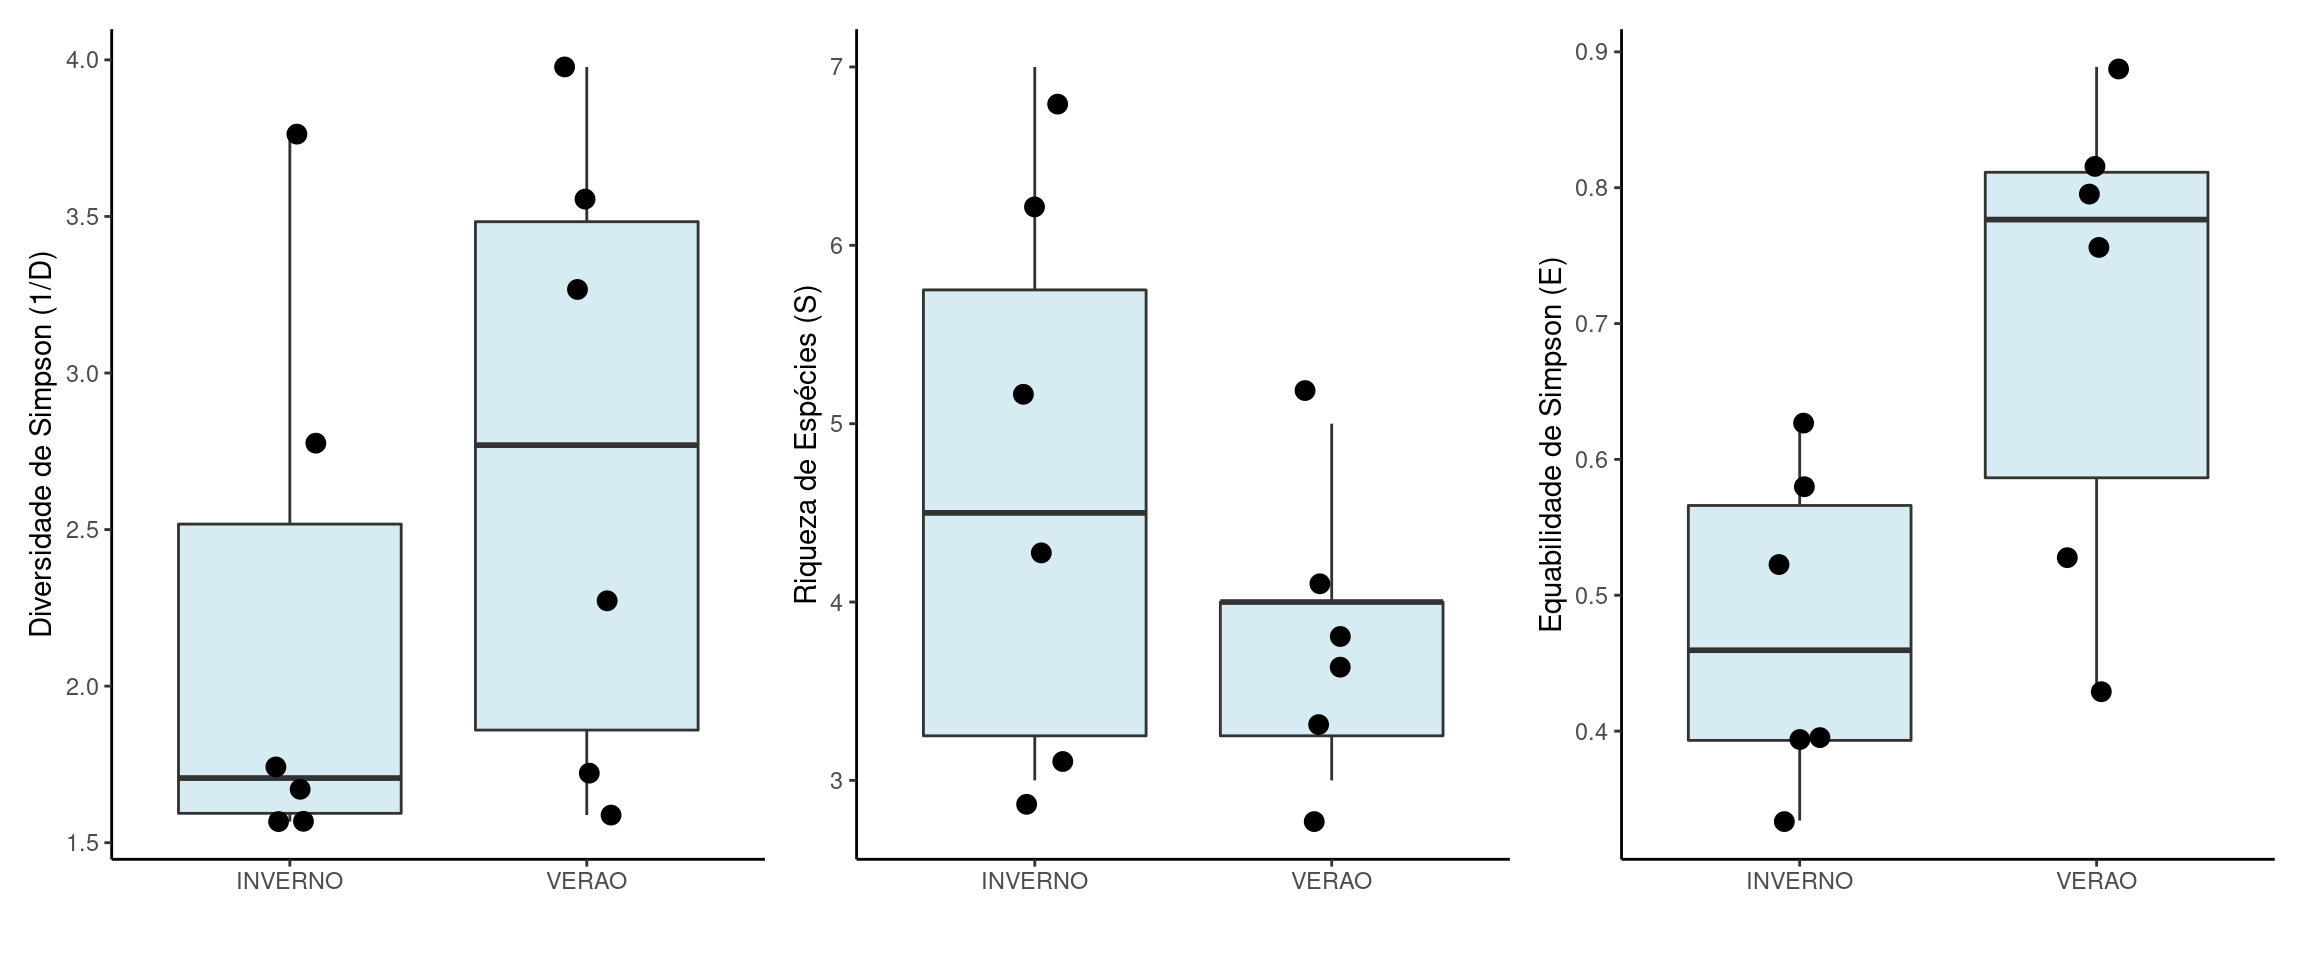
\includegraphics{medidas-diversidade_files/figure-latex/unnamed-chunk-25-1} \end{center}

\begin{quote}
Para visualizar os gráficos lado-a-lado com o comando acima você deve ter instalado e habilitado o pacote \texttt{patchwork}.
\end{quote}

Note que é importante observar os três componentes da diversidade. Nas figuras, a diversidade medida pelo índice de Simpson parace mair elevada no período do VERAO. Entretanto a riqueza parece menor neste período, sugerindo que a elevada diversidade foi observada principalmente por influência da equabilidade, claramente mais elevada no VERAO. Deste modo, embora no período do inverno tenham apareceido em média mais espécies, a dominânca também foi maior, isto é, algumas espécies são desproporcionalmente mais abundantes que o restante nas comunidades.

\begin{quote}
\emph{Para detalhes sobre o boxplot, veja o link:} Estatística nas Ciências Ambientais - Capítulos 7 e 11
\end{quote}

\hypertarget{diversidade-gamma}{%
\section{\texorpdfstring{Diversidade \(\gamma\)}{Diversidade \textbackslash gamma}}\label{diversidade-gamma}}

A princípio, a diversidade \(\gamma\) pode ser medida com qualquer um dos índices utilizados para descrever a diversidade \(\alpha\), bastando para isto somar as abundâncias das espécies em todos os pontos. Entretanto, quando olhamos para a diversidade total uma pergunta que devemos nos fazer é:

\begin{quote}
O número de amostras que tenho em mãos parece ter sido suficiente para caracterizar a comunidade?
\end{quote}

É esperado por exemplo que ao adicionamos novas amostras locais, a riqueza de espécies também total aumente. Em nosso exemplo, se tivéssemos somente uma amostra, certamente não veríamos todas as \(10\) espécies de nossa matriz. Ao adicionar uma segunda amostra, novas espécies não observadas na primeira podem surgir, fazendo com que o número total aumente. À medida que continuamos adicionando amostras novas, é esperado que outras espécias vão sendo acumuladas no cômputo total. Entretanto, em algum momento, é esperado que já tenhamos observado todas as espécies e, a partir daí, a adição de novas amostras não trará nenhuma espécies que já não tenha sido observada. Neste momento, saberemos que a comunidade foi adequadamente caracterizada por sua riqueza total.

Para verificarmos como o número de espécies total aumenta com o número de amostras locais podemos construir uma \textbf{curva de acumulação de espécies} ou \textbf{curva do coletor}. Se fizermos isto para as seis amostras do VERAO teríamos:

\begin{Shaded}
\begin{Highlighting}[]
\NormalTok{ac\_verao }\OtherTok{=}\NormalTok{ pe }\SpecialCharTok{\%\textgreater{}\%} 
  \FunctionTok{filter}\NormalTok{(Epoca }\SpecialCharTok{==} \StringTok{\textquotesingle{}VERAO\textquotesingle{}}\NormalTok{) }\SpecialCharTok{\%\textgreater{}\%}
  \FunctionTok{select}\NormalTok{(}\SpecialCharTok{{-}}\NormalTok{Epoca) }\SpecialCharTok{\%\textgreater{}\%} 
  \FunctionTok{specaccum}\NormalTok{(}\AttributeTok{method =} \StringTok{\textquotesingle{}collector\textquotesingle{}}\NormalTok{)}

\FunctionTok{plot}\NormalTok{(}\AttributeTok{y =}\NormalTok{ ac\_verao}\SpecialCharTok{$}\NormalTok{richness, }\AttributeTok{x =}\NormalTok{ ac\_verao}\SpecialCharTok{$}\NormalTok{sites,}
     \AttributeTok{type =} \StringTok{\textquotesingle{}b\textquotesingle{}}\NormalTok{, }\AttributeTok{pch =} \DecValTok{19}\NormalTok{, }\AttributeTok{col =} \DecValTok{2}\NormalTok{, }\AttributeTok{lty =} \DecValTok{2}\NormalTok{,}
     \AttributeTok{ylab =} \StringTok{\textquotesingle{}Riqueza acumulada\textquotesingle{}}\NormalTok{,}
     \AttributeTok{xlab =} \StringTok{\textquotesingle{}Número de amostras\textquotesingle{}}\NormalTok{)}
\end{Highlighting}
\end{Shaded}

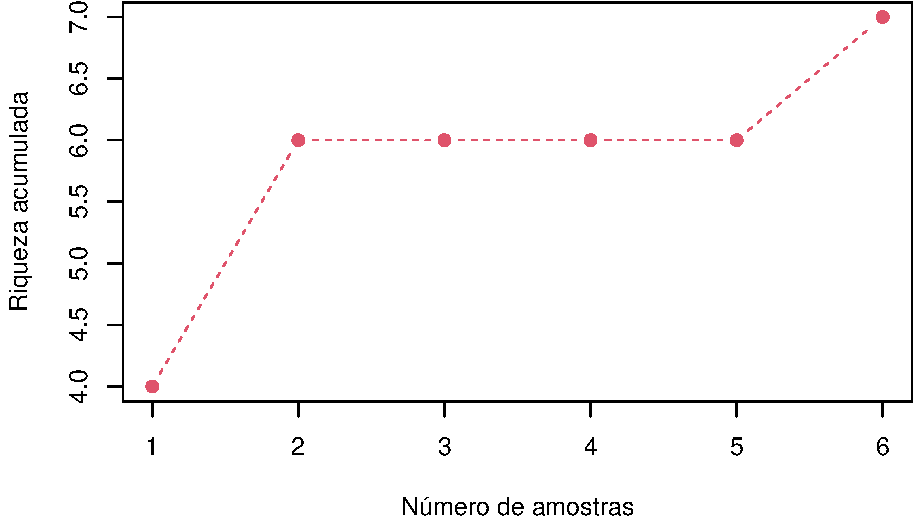
\includegraphics{medidas-diversidade_files/figure-latex/unnamed-chunk-26-1.pdf}

Esta figura mostra que na primeira amostra do verão foram observadas \(4\) espécies. Ao adicionar a segunda amostra, verificamos duas espécies adicionais, totalizando \(6\) espécies. Nenhuma espécie adicional foi observada da \(3^a\) a \(5^a\) amostra e somente na \(6^a\) amostra, mais uma espécie foi observada, totalizando \(7\) espécies observadas no período do VERAO.

A figura mostrada acima seguiu exatamente a sequência de amostras das linhas de nossa tabela, simplesmente pois foi a sequência registrada na base de dados. No entanto qualquer outra sequência seria igualamente válida. Assim, para termos um padrão \textbf{esperado}, existem vários métodos que nos permitirão encontrar uma valor de riqueza \textbf{médio} como função do número de amostras.

A mesma ideia pode ser reformulada pensando na adição de indivíduos, isto é: a partir de quantos indivíduos amostrados a comunidade terá sua riqueza adaquadamente caracterizada?

Vamos avalir esta questão para nossas comunidades de VERAO e de INVERNO, construindo curvas de acumulação para a riqueza de espécies como função do número de indivíduos nas amostras. Pàra isto, vamos utilizar o pacote iNEXT.

Inicialmente, precisamos criar uma lista separando as comunidades de verão e inverno:

\begin{Shaded}
\begin{Highlighting}[]
\NormalTok{pe\_list }\OtherTok{=} \FunctionTok{list}\NormalTok{()}
\NormalTok{pe\_list}\SpecialCharTok{$}\NormalTok{VERAO }\OtherTok{=}\NormalTok{ pe }\SpecialCharTok{\%\textgreater{}\%} 
  \FunctionTok{filter}\NormalTok{(Epoca }\SpecialCharTok{==} \StringTok{\textquotesingle{}VERAO\textquotesingle{}}\NormalTok{) }\SpecialCharTok{\%\textgreater{}\%} 
  \FunctionTok{select}\NormalTok{(}\SpecialCharTok{{-}}\NormalTok{Epoca) }\SpecialCharTok{\%\textgreater{}\%} 
  \FunctionTok{colSums}\NormalTok{()}
  
\NormalTok{pe\_list}\SpecialCharTok{$}\NormalTok{INVERNO }\OtherTok{=}\NormalTok{ pe }\SpecialCharTok{\%\textgreater{}\%} 
  \FunctionTok{filter}\NormalTok{(Epoca }\SpecialCharTok{==} \StringTok{\textquotesingle{}INVERNO\textquotesingle{}}\NormalTok{) }\SpecialCharTok{\%\textgreater{}\%} 
  \FunctionTok{select}\NormalTok{(}\SpecialCharTok{{-}}\NormalTok{Epoca) }\SpecialCharTok{\%\textgreater{}\%} 
  \FunctionTok{colSums}\NormalTok{()}
\end{Highlighting}
\end{Shaded}

Em seguida, utilizamos a função \texttt{iNEXT}, com os argumentos \texttt{datatype\ =\ \textquotesingle{}abundance\textquotesingle{}} (indivíduos no eixo \(x\)) e \texttt{q\ =\ 0} (riqueza acumulada no eixo \(y\)).

\begin{Shaded}
\begin{Highlighting}[]
\NormalTok{gama\_ac }\OtherTok{\textless{}{-}} \FunctionTok{iNEXT}\NormalTok{(pe\_list, }
                 \AttributeTok{datatype =} \StringTok{\textquotesingle{}abundance\textquotesingle{}}\NormalTok{, }
                 \AttributeTok{q =} \DecValTok{0}\NormalTok{)}

\NormalTok{plt\_nbreadth }\OtherTok{\textless{}{-}} \FunctionTok{ggiNEXT}\NormalTok{(gama\_ac) }\SpecialCharTok{+}
  \FunctionTok{labs}\NormalTok{(}\AttributeTok{y =} \StringTok{\textquotesingle{}Riqueza acumulada\textquotesingle{}}\NormalTok{,}
       \AttributeTok{x =} \StringTok{\textquotesingle{}Número de indivíduos\textquotesingle{}}\NormalTok{) }\SpecialCharTok{+}
  \FunctionTok{theme\_classic}\NormalTok{() }\SpecialCharTok{+}
  \FunctionTok{scale\_y\_continuous}\NormalTok{(}\AttributeTok{breaks =} \DecValTok{0}\SpecialCharTok{:}\DecValTok{10}\NormalTok{) }\SpecialCharTok{+}
  \FunctionTok{theme}\NormalTok{(}\AttributeTok{legend.position =} \StringTok{"bottom"}\NormalTok{, }
        \AttributeTok{legend.title=}\FunctionTok{element\_blank}\NormalTok{())}
\end{Highlighting}
\end{Shaded}

\begin{Shaded}
\begin{Highlighting}[]
\NormalTok{plt\_nbreadth}
\end{Highlighting}
\end{Shaded}

\begin{center}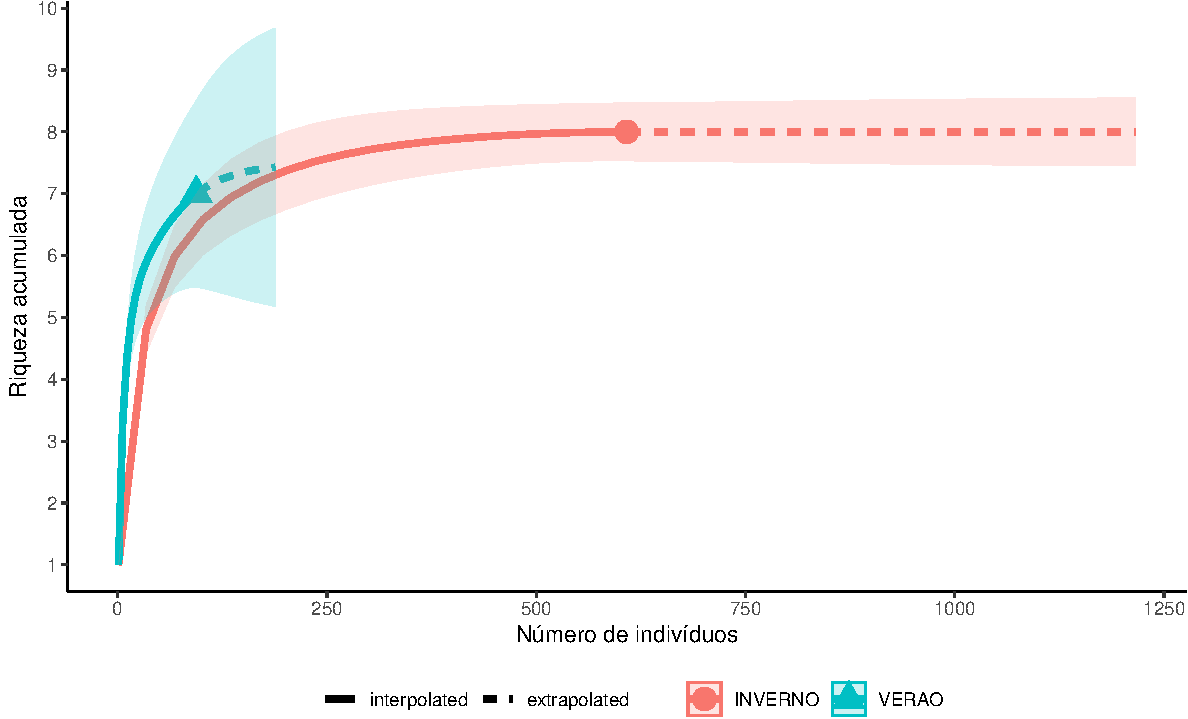
\includegraphics{medidas-diversidade_files/figure-latex/unnamed-chunk-29-1} \end{center}

O método do pacote \texttt{iNEXT} permite fazermos uma \textbf{extrapolação} do que seria esperado. Desta figura pércebemos dois ponto importantes.

\begin{itemize}
\item
  a riqueza total é similar entre os períodos, ainda que localmente, o verão tenha tido em média menor riqueza (veja padrões de diversidade \(\alpha\)).
\item
  A comunidade de INVERNO tem mais indivíduos e aparentemente foi bem caracterizada, uma vez que a riqueza de espécies acumulada parece se estabilizar ao redor de 8 espécies. A comunidade de VERAO por outro lado, teve poucos indivíduos amostrados, de modo que ainda não há informação o suficiente para sabermos o que poderia acontecer caso continuássemos a amostrar as comunidades neste período. Esta incerteza pode ser observada na larga faixa em verde que contrasta com a faixa em vermelho menos estreita.
\end{itemize}

\hypertarget{diversidade-beta}{%
\section{\texorpdfstring{Diversidade \(\beta\)}{Diversidade \textbackslash beta}}\label{diversidade-beta}}

\hypertarget{salvando-as-figuras-deste-tutorial}{%
\section{Salvando as figuras deste tutorial}\label{salvando-as-figuras-deste-tutorial}}

  \bibliography{book.bib,packages.bib}

\end{document}
